\documentclass[12pt]{article}

\usepackage[margin=1in]{geometry}
\usepackage{graphicx}
\usepackage{hyperref}
\usepackage{lineno}
\usepackage{natbib}
\usepackage{setspace}
\usepackage{tikz}

\usetikzlibrary{arrows.meta, calc, fit, positioning}

\hypersetup{
  colorlinks=true,
  linkcolor=black,
  citecolor=black,
  urlcolor=black
}
\emergencystretch=2em

\linenumbers
\doublespacing

\title{TCGA-TRACE: auditable survival analysis for TCGA transcriptomic biomarkers}
\author{
  Sergio Hernández-Galaz$^{1,2,3}$,
  Andrés Hernández-Oliveras$^{1,2}$,
  Ignacio Pezoa-Soto$^{1,3,4}$,\\
  Javiera Reyes-Alvarez$^{1}$,
  Vincenzo Benedetti$^{1}$,\\
  Alberto J. M. Martin$^{1,4}$, and
  Alvaro Lladser$^{1,3}$\\
  $^{1}$Centro BASAL Ciencia \& Vida, Fundación Ciencia \& Vida, Santiago, Chile.\\
  $^{2}$Fundación Arturo López Pérez (FALP), OECI Cancer Center,
  Laboratorio de Medicina Traslacional, Centro de Investigación e Innovación
  en Cáncer, Santiago, Chile.\\
  $^{3}$Facultad de Medicina, Universidad San Sebastián, Santiago, Chile.\\
  $^{4}$Escuela de Ingeniería, Facultad de Ingeniería,
  Universidad San Sebastián, Santiago, Chile.\\
  Correspondence: email@example.org
}
\date{}

\begin{document}
\maketitle

\begin{abstract}
\noindent
\textbf{Summary:}
Interactive TCGA survival results are difficult to audit when cohort,
expression and model decisions are detached from the output. TCGA-TRACE
combines continuous Cox and spline models, grouped sensitivities, signatures,
interactions and pan-cancer analysis with a prespecified
endpoint--score--cutpoint multiverse, an optional post hoc session history and
a server-signed, reconstructable record of participants, expression, sources,
software and results; six isolated reruns reproduced frozen outputs, three
literature-aligned cases were directionally concordant and one RNA interaction
remained unsupported, while the complete panel retained null and discordant
results.
\textbf{Availability and Implementation:}
The registration-free service is available at
\url{https://apps.cienciavida.org/tcga_explorer/}. Source code and
reproducibility materials are at
\url{https://github.com/lladserLab/tcga_explorer}; the exact submitted release,
benchmarks and 33-cohort snapshot manifest are archived at
\texttt{ARCHIVE-DOI-PENDING}. The Dockerized application uses FastAPI, React
and R.
\textbf{Contact:} email@example.org.
\textbf{Supplementary information:} Supplementary data are available with the
manuscript.
\end{abstract}

\section{Introduction}

Transcriptomic survival associations can prioritize hypotheses, but their
apparent strength depends on endpoint, eligibility, RNA-sample selection,
expression scale, cutpoint and model. Outcome-optimized cutpoints are
particularly vulnerable when alternatives are hidden
\citep{altmanRoyston2006}.

Established resources cover complementary parts of this workflow: GEPIA2
supports gene, isoform and signature survival \citep{gepia22019}; cSurvival
implements two-predictor cutoff searches \citep{csurvival2022}; PESSA provides
ssGSEA, continuous/grouped Cox and Schoenfeld tests \citep{pessa2024}. Other
portals and code workflows expand assay, dataset or programming breadth
(Supplementary Table S1). These methods are prior art. The narrower unresolved
problem is exporting the exact endpoint, participants, RNA samples, score
construction, diagnostics, multiplicity scope and software as one
reconstructable run.

TCGA-TRACE was developed for researchers evaluating transcriptomic survival
hypotheses. It connects endpoint-aware cohorts to single-gene, signature,
interaction and pan-cancer analyses. Rather than proposing a new estimator, it
provides a verifiable run record and prespecified specification curve;
Supplementary Table S1 compares representative resources, and
Figure~\ref{fig:trace-workflow} summarizes the reporting workflow.

\begin{figure*}[!t]
\centering
\resizebox{\textwidth}{!}{%
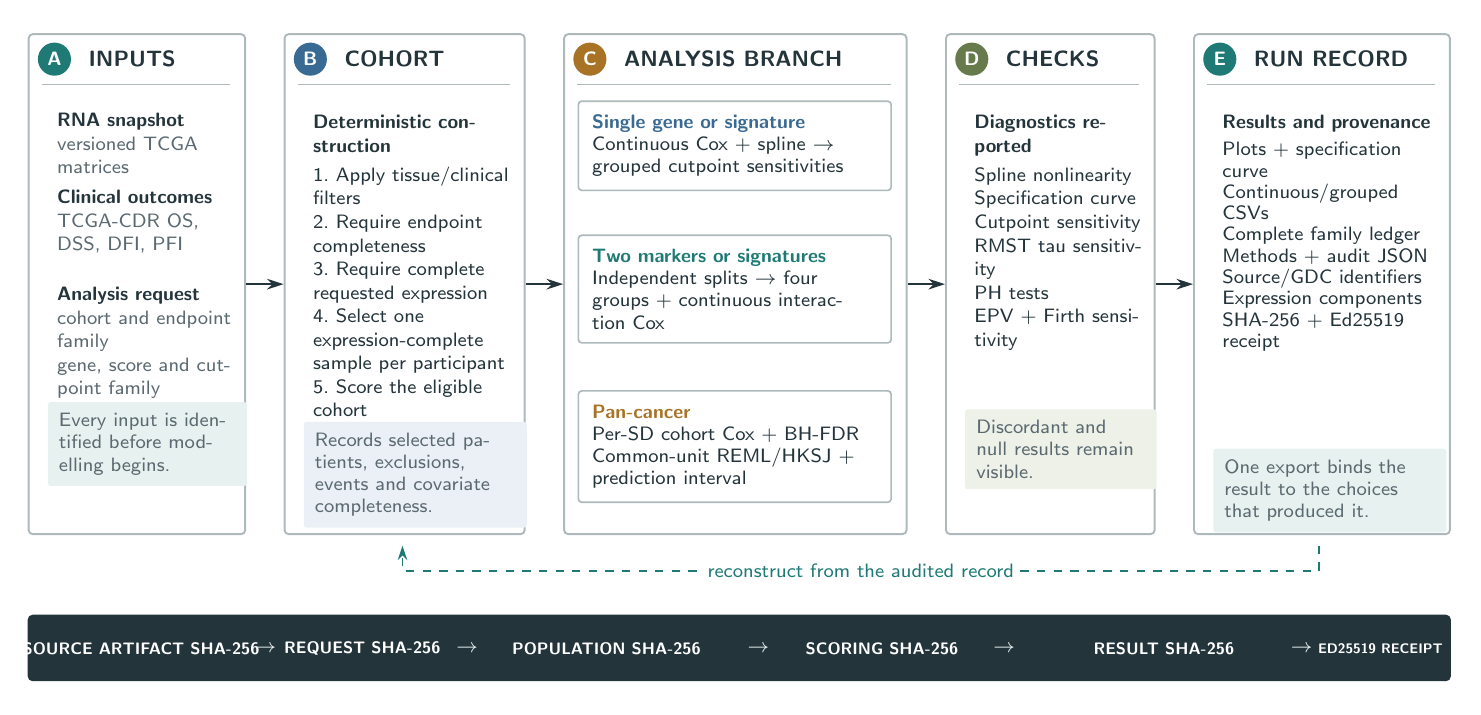
\begin{tikzpicture}[x=1cm,y=1cm]
\definecolor{traceInk}{HTML}{24343B}
\definecolor{traceMuted}{HTML}{5B6970}
\definecolor{traceLine}{HTML}{AEB9BC}
\definecolor{traceTeal}{HTML}{1F7A75}
\definecolor{traceTealLight}{HTML}{E7F2F0}
\definecolor{traceBlue}{HTML}{396A93}
\definecolor{traceBlueLight}{HTML}{EAF0F5}
\definecolor{traceAmber}{HTML}{A87325}
\definecolor{traceAmberLight}{HTML}{F7F0E4}
\definecolor{traceOlive}{HTML}{667A4C}
\definecolor{traceOliveLight}{HTML}{EDF1E8}

\tikzset{
  panel/.style={
    draw=traceLine,
    fill=white,
    line width=0.7pt,
    rounded corners=1.5pt
  },
  branch/.style={
    draw=traceLine,
    fill=white,
    line width=0.6pt,
    rounded corners=1.2pt,
    align=left,
    inner sep=5pt,
    font=\sffamily\fontsize{6.8}{8.0}\selectfont,
    text=traceInk
  },
  stage title/.style={
    anchor=west,
    font=\sffamily\bfseries\fontsize{8.2}{9.2}\selectfont,
    text=traceInk
  },
  stage number/.style={
    circle,
    minimum size=0.42cm,
    inner sep=0pt,
    font=\sffamily\bfseries\fontsize{7.3}{8}\selectfont,
    text=white
  },
  item/.style={
    anchor=north west,
    align=left,
    font=\sffamily\fontsize{7.2}{8.5}\selectfont,
    text=traceInk
  },
  small/.style={
    anchor=north west,
    align=left,
    font=\sffamily\fontsize{6.8}{8.0}\selectfont,
    text=traceMuted
  },
  flow/.style={
    -{Stealth[length=2.1mm,width=1.35mm]},
    draw=traceInk,
    line width=0.75pt
  }
}

\path[use as bounding box] (0,0.05) rectangle (18.1,8.42);

% A. Inputs
\node[panel, minimum width=2.75cm, minimum height=6.35cm, anchor=north west] (inputs) at (0,8.35) {};
\node[stage number, fill=traceTeal] at (0.34,8.02) {A};
\node[stage title] at (0.65,8.02) {INPUTS};
\draw[traceLine, line width=0.45pt] (0.18,7.70) -- (2.57,7.70);
\node[item, text width=2.25cm] at (0.25,7.46) {
  \textbf{RNA snapshot}\\
  \textcolor{traceMuted}{versioned TCGA matrices}
};
\node[item, text width=2.25cm] at (0.25,6.48) {
  \textbf{Clinical outcomes}\\
  \textcolor{traceMuted}{TCGA-CDR OS, DSS, DFI, PFI}
};
\node[item, text width=2.25cm] at (0.25,5.25) {
  \textbf{Analysis request}\\
  \textcolor{traceMuted}{cohort and endpoint family}\\
  \textcolor{traceMuted}{gene, score and cutpoint family}\\
  \textcolor{traceMuted}{filters and model choices}
};
\node[small, text width=2.25cm, fill=traceTealLight, rounded corners=1pt, inner sep=4pt]
  at (0.25,3.67) {Every input is identified before modelling begins.};

% B. Deterministic cohort construction
\node[panel, minimum width=3.05cm, minimum height=6.35cm, anchor=north west] (cohort) at (3.25,8.35) {};
\node[stage number, fill=traceBlue] at (3.59,8.02) {B};
\node[stage title] at (3.90,8.02) {COHORT};
\draw[traceLine, line width=0.45pt] (3.43,7.70) -- (6.12,7.70);
\node[item, text width=2.55cm] at (3.50,7.43) {
  \textbf{Deterministic construction}\\[2pt]
  1.\ Apply tissue/clinical filters\\
  2.\ Require endpoint completeness\\
  3.\ Require complete requested expression\\
  4.\ Select one expression-complete sample per participant\\
  5.\ Score the eligible cohort
};
\node[small, text width=2.55cm, fill=traceBlueLight, rounded corners=1pt, inner sep=4pt]
  at (3.50,3.42) {
  Records selected patients, exclusions, events and covariate completeness.
};

% C. Analysis branches
\node[panel, minimum width=4.35cm, minimum height=6.35cm, anchor=north west] (analysis) at (6.80,8.35) {};
\node[stage number, fill=traceAmber] at (7.14,8.02) {C};
\node[stage title] at (7.45,8.02) {ANALYSIS BRANCH};
\draw[traceLine, line width=0.45pt] (6.98,7.70) -- (10.97,7.70);
\node[branch, text width=3.62cm] (single) at (8.98,6.92) {
  \textbf{\textcolor{traceBlue}{Single gene or signature}}\\
  Continuous Cox + spline $\rightarrow$ grouped cutpoint sensitivities
};
\node[branch, text width=3.62cm] (crossed) at (8.98,5.10) {
  \textbf{\textcolor{traceTeal}{Two markers or signatures}}\\
  Independent splits $\rightarrow$ four groups + continuous interaction Cox
};
\node[branch, text width=3.62cm] (pancancer) at (8.98,3.10) {
  \textbf{\textcolor{traceAmber}{Pan-cancer}}\\
  Per-SD cohort Cox + BH-FDR\\
  Common-unit REML/HKSJ + prediction interval
};

% D. Diagnostics
\node[panel, minimum width=2.65cm, minimum height=6.35cm, anchor=north west] (diagnostics) at (11.65,8.35) {};
\node[stage number, fill=traceOlive] at (11.99,8.02) {D};
\node[stage title] at (12.30,8.02) {CHECKS};
\draw[traceLine, line width=0.45pt] (11.83,7.70) -- (14.12,7.70);
\node[item, text width=2.15cm] at (11.90,7.43) {
  \textbf{Diagnostics reported}\\[2pt]
  Spline nonlinearity\\
  Specification curve\\
  Cutpoint sensitivity\\
  RMST tau sensitivity\\
  PH tests\\
  EPV + Firth sensitivity
};
\node[small, text width=2.15cm, fill=traceOliveLight, rounded corners=1pt, inner sep=4pt]
  at (11.90,3.58) {Discordant and null results remain visible.};

% E. Exported record
\node[panel, minimum width=3.25cm, minimum height=6.35cm, anchor=north west] (export) at (14.80,8.35) {};
\node[stage number, fill=traceTeal] at (15.14,8.02) {E};
\node[stage title] at (15.45,8.02) {RUN RECORD};
\draw[traceLine, line width=0.45pt] (14.98,7.70) -- (17.87,7.70);
\node[item, text width=2.68cm,
  font=\sffamily\fontsize{6.6}{7.7}\selectfont] at (15.05,7.43) {
  \textbf{Results and provenance}\\[2pt]
  Plots + specification curve\\
  Continuous/grouped CSVs\\
  Complete family ledger\\
  Methods + audit JSON\\
  Source/GDC identifiers\\
  Expression components\\
  SHA-256 + Ed25519 receipt
};
\node[small, text width=2.68cm, fill=traceTealLight, rounded corners=1pt, inner sep=4pt]
  at (15.05,3.08) {One export binds the result to the choices that produced it.};

% Main flow
\draw[flow] (inputs.east) -- (cohort.west);
\draw[flow] (cohort.east) -- (analysis.west);
\draw[flow] (analysis.east) -- (diagnostics.west);
\draw[flow] (diagnostics.east) -- (export.west);

% Re-execution loop
\draw[-{Stealth[length=1.8mm,width=1.2mm]}, draw=traceTeal, line width=0.65pt, dashed]
  (16.40,1.84) -- (16.40,1.52) -- (4.76,1.52) -- (4.76,1.84);
\node[font=\sffamily\fontsize{6.7}{7.5}\selectfont, text=traceTeal, fill=white, inner sep=1.5pt]
  at (10.58,1.52) {reconstruct from the audited record};

% Provenance rail
\node[panel, fill=traceInk, draw=traceInk, minimum width=18.05cm, minimum height=0.82cm, anchor=south west]
  (rail) at (0,0.12) {};
\node[font=\sffamily\bfseries\fontsize{5.8}{6.6}\selectfont, text=white]
  at (1.44,0.53) {SOURCE ARTIFACT SHA-256};
\node[font=\sffamily\bfseries\fontsize{7}{7.5}\selectfont, text=traceTealLight] at (3.02,0.53) {$\rightarrow$};
\node[font=\sffamily\bfseries\fontsize{5.8}{6.6}\selectfont, text=white]
  at (4.25,0.53) {REQUEST SHA-256};
\node[font=\sffamily\bfseries\fontsize{7}{7.5}\selectfont, text=traceTealLight] at (5.58,0.53) {$\rightarrow$};
\node[font=\sffamily\bfseries\fontsize{5.8}{6.6}\selectfont, text=white]
  at (7.35,0.53) {POPULATION SHA-256};
\node[font=\sffamily\bfseries\fontsize{7}{7.5}\selectfont, text=traceTealLight] at (9.28,0.53) {$\rightarrow$};
\node[font=\sffamily\bfseries\fontsize{5.8}{6.6}\selectfont, text=white]
  at (10.85,0.53) {SCORING SHA-256};
\node[font=\sffamily\bfseries\fontsize{7}{7.5}\selectfont, text=traceTealLight] at (12.40,0.53) {$\rightarrow$};
\node[font=\sffamily\bfseries\fontsize{5.8}{6.6}\selectfont, text=white]
  at (14.43,0.53) {RESULT SHA-256};
\node[font=\sffamily\bfseries\fontsize{7}{7.5}\selectfont, text=traceTealLight] at (16.18,0.53) {$\rightarrow$};
\node[font=\sffamily\bfseries\fontsize{5.2}{6.0}\selectfont, text=white]
  at (17.18,0.53) {ED25519 RECEIPT};
\end{tikzpicture}%
}

\caption{TCGA-TRACE links versioned RNA and outcome data to deterministic
participant-level cohort construction, continuous and grouped survival
analyses, model diagnostics and a server-signed run record. The exported record
supports reconstruction of scores and statistical outputs and verification of
its server origin.
\textbf{Alt text:} A five-stage flow diagram connects TCGA inputs, cohort
construction, three analysis branches, diagnostic checks and an exported run
record. A SHA-256 provenance rail links source, request, population, scoring
and result hashes to a detached Ed25519 receipt.}
\label{fig:trace-workflow}
\end{figure*}

\section{Methods}

\subsection{Data and cohort construction}

TCGA-TRACE links retrospective bulk RNA-seq matrices from the Genomic Data
Commons \citep{gdcDataset2026} to TCGA-CDR overall survival (OS),
disease-specific survival (DSS), disease-free interval (DFI) and
progression-free interval (PFI) \citep{liu2018tcga}. Endpoints
require at least 10 linked participants and five events as operational QC.
After filters and endpoint completeness, the requested score is required before
a documented biospecimen rule selects one expression-complete RNA sample per
participant. Adjusted models repeat the 10-participant/five-event check after
complete-case filtering.
For DSS, DFI and PFI, TCGA-CDR status 0/1/2 denotes censoring, the endpoint
event and an endpoint-specific competing death. Kaplan--Meier/Cox censor code
2, whereas companion cumulative-incidence, Gray-test and Fine--Gray outputs
retain it; cause-specific HRs and subdistribution HRs are reported as distinct
estimands.

\subsection{Survival analyses}

Inputs may be individual genes or signatures scored by the mean, z-score or
weighted method (Supplementary Table S2). Z-score signatures standardize genes
among eligible participants; because eligibility changes with endpoint and
filters, their numerical scores are not transportable across runs. Weighted
scores use \(\sum_g w_g x_{ig}/\sum_g |w_g|\). The primary analysis reports a
Cox HR per score SD. A three-degree-of-freedom restricted cubic spline
(percentile knots 5, 35, 65 and 95) tests nonlinearity by likelihood-ratio test
and reports a median-referenced 5th--95th-percentile profile; it requires 20
participants and 15 events.

Grouping options are median, tertiles, upper or outer quartiles, custom
percentile and maximally selected rank statistics. Secondary Kaplan--Meier,
log-rank, grouped Cox and restricted mean survival time (RMST) outputs label
maxstat as outcome-optimized. Lau94 adjusts its rank-test \(p\), but grouped HR,
confidence interval and RMST remain post-selection. The benchmark compares four
nonredundant two-group rules (maxstat, median, upper and outer quartiles);
tertiles are three-group and custom percentiles are user-defined. Their
\(p\)-values form a within-scenario Holm family, using Lau94 for maxstat. BH is
applied separately across 11 linear and 11 spline-nonlinearity hypotheses.
The 11 scenarios were assembled after exploratory triage and then frozen in a
versioned registry; this is a heterogeneous software stress test, not
prospective biomarker selection. OS is the registered primary endpoint except
for UVM BAP1 DSS, while BRCA MKI67 PFI and LUAD CD274 PFI are linked endpoint
sensitivities that cannot replace their OS parent because of observed results.

Continuous and grouped Cox models use Efron handling of ties. Users may
prespecify an exact complete-case adjustment using age per 10 years, ordinal
stage or grade, and categorical GDC gender or race; unavailable models are not
replaced. Marker-term and global \texttt{cox.zph} tests are separate
interpretation cautions, never exclusion rules. When marker-term \(p<0.05\), a
diagnostic counting-process Cox model reports marker HRs before and after a
fixed two-year split and their ratio, using Efron ties, participant-clustered
robust variance, at least five events per period and 10 participants entering
the late period. The group-independent RMST horizon is the smaller of five years
and the eligible cohort's 75th
endpoint-time percentile, requires five participants at risk per group and has
0.75/0.90 sensitivities. Cox outputs report fitted
parameters and events per parameter, cautioning below 10 and severely below 5.
Low-information, unstable, non-finite or extreme fits add, but do not substitute,
a Firth/\texttt{coxphf} sensitivity. Crossed
signatures report stratified groups and a continuous z-scored interaction.

Pan-cancer cohort models report a descriptive HR per within-cohort expression
SD and do not pool these cohort-specific increments. Eligible single-gene,
mean or weighted effects are recovered per common input-score unit and
synthesized only within one endpoint and model family using REML,
Hartung--Knapp--Sidik--Jonkman inference and a 95\% prediction interval.
Z-score signatures, mixed endpoints and availability-selected adjustment
families are not pooled.

\subsection{Web server and run record}

The React interface calls a Python/FastAPI backend that constructs cohorts and
invokes R. A multiverse freezes up to 72 endpoint--score--cutpoint
specifications before execution. Unique endpoint--score Cox tests and grouped
sensitivities form separate multiplicity families. Every planned cell,
including failures, retains request, child-analysis and audit hashes; PH is not
a filter and no binary verdict is calculated.
Outside a declared multiverse, an opt-in browser-local history exports up to
200 selected events that reference terminal jobs. It deduplicates exact
hypotheses and separates
continuous, grouped and interaction multiplicity families; multiverse and
pan-cancer corrections are referenced without recounting. This post hoc scope
cannot attest that no other runs occurred.
Operating characteristics were evaluated separately by permuting expression
2,000 times in a frozen observed cohort and simulating 2,000 datasets of
\(n=300\) under null, linear PH, delayed non-PH and U-shaped effects. Each
replicate refitted continuous Cox, spline, marker PH and four grouped rules;
rejection proportions have Wilson 95\% intervals.

Each run exports de-identified participant records, endpoint source,
exclusions, expression-artifact hashes, GDC identifiers, gene components,
standardization parameters, software and results. Separate hashes bind
continuous and grouped populations. Two-group exports add patient-level input,
a standalone R runner, \texttt{renv.lock} and an immutable-base Dockerfile. The
verifier recomputes hashes, reconstructs scores and reruns the frozen input,
adapting REMARK principles to exploratory web analysis.
A detached Ed25519 receipt signs the exact audit bytes, schema and recorded run
hash. The public key is exposed through the HTTPS API and archived with the
benchmark; verification establishes server origin under that trusted key, not
scientific correctness or append-only publication time.

\section{Case Studies and Evaluation}

\subsection*{Technical validation}

Three frozen exports---single-gene (365 participants), weighted-signature (79)
and crossed-signature (80)---passed reconstruction checks. Six isolated
arm64/amd64 capsule reruns matched core outputs under quantity-specific
tolerances (Supplementary Table S3), and Ed25519 verification detected altered
audit bytes even after internal hashes were recomputed. This threat model
addresses accidental drift and unverifiable origin, not fraud by a trusted
signing service.

The complete registered panel, rather than the examples selected for exposition,
retains supported, unsupported, nonlinear, sparse-event and PH-discordant
results (Supplementary Table S4). Six of 11 linear effects and two spline tests
had BH \(q<0.05\); grouped Holm support was 4/4 in five scenarios, 3/4 in one
and 0/4 in five. Maxstat increased absolute log-HR relative to the median in all
10 estimable scenarios (median ratio 1.80). EMP3/LGG showed an attenuating
two-period effect, while CA9/KIRC was nonlinear despite unsupported linear and
grouped tests. A three-case cBioPortal comparison likewise retained full
agreement, direction-only agreement and a jointly unsupported result. Because
the following four cases were chosen post hoc for explanation, they do not
replace the frozen panel or define an inferential family.

\subsection{Case 1: CDC20 in Hepatocellular Cancer}

A published CDC20--FCN3 model associated CDC20 with survival in TCGA and ICGC
hepatocellular carcinoma \citep{lai2022cdc20}. TCGA-TRACE tested CDC20 alone:
365 participants and 130 events gave HR/SD 1.65 (1.38--1.98), age-adjusted HR
1.67 (1.39--2.01), support under all four grouped rules and median-split RMST
difference -207 days at \(\tau=1091\) days. This is directional workflow
concordance, not independent validation, because the source study also used
TCGA and its two-gene model was not reconstructed.

\subsection{Case 2: BUB1B--PINK1 in ACC}

In an independent Brazilian qRT-PCR cohort, BUB1B combined with PINK1 was the
strongest reported overall-survival predictor among adult adrenocortical
carcinomas \citep{fragoso2012bub1b}. The TCGA RNA-seq analogue
\((\mathrm{BUB1B}-\mathrm{PINK1})/2\) gave HR/SD 2.85 (1.90--4.26) in 79
participants with 28 events and stage-adjusted HR 2.15 (1.42--3.26). A median
split gave HR 4.12 (1.75--9.71), stage-adjusted HR 3.54 (1.47--8.51) and RMST
difference -460 days at \(\tau=1826\) days (Supplementary Table S5). This
cross-cohort, cross-assay agreement corroborates direction; it does not reproduce
the original assay or threshold.

\subsection{Case 3: BIRC5 Across TCGA Cohorts}

A prior 33-cancer study linked higher BIRC5 expression to worse OS in 14 cancer
types and reported external support in breast, lung and gastric datasets
\citep{faldtBeding2022birc5}. TCGA-TRACE found 18/32 cohort effects at
FDR \(<0.10\) and common-scale REML HR 1.20 (HKSJ 95\% CI 1.06--1.37).
The stage-adjusted family had the same mean direction, but \(I^2=86.1\%\) and
prediction intervals crossed 1 (primary 0.64--2.24; stage-adjusted 0.73--1.98).
This is within-TCGA literature concordance, not independent validation; the
heterogeneity and prediction intervals do not support a universal effect
across cancers (Supplementary Tables S5--S6).

\subsection{Case 4: BAP1/PRAME in Uveal Melanoma}

This was the deliberately non-confirmatory case. Published immunohistochemistry
in 318 uveal melanomas stratified metastatic and disease-specific risk using
BAP1 and PRAME \citep{han2023bap1prame}. TCGA RNA-expression groups differed
globally (\(p=0.002\)), but the continuous interaction was unsupported
(\(p=0.637\)); with 21 events, its age-adjusted Firth sensitivity was also
unsupported (\(p=0.126\)). Group separation therefore neither establishes an
RNA interaction nor reproduces the protein assay.

\subsection{Calibration and Runtime}

Under observed-cohort expression permutation, rejection proportions were
5.0\% for linear Cox, 5.8\% for spline nonlinearity, 5.1\% for marker PH and
3.2\% for the grouped Holm family. Naive maxstat rejected 39.6\%, versus
1.8\% for Lau94. Marker PH detected 88.2\% of delayed effects and the spline
detected 100\% of U-shaped effects in known-truth simulations (Supplementary
Table S7); these are separate operating characteristics, not votes.

On an Apple M1 Ultra Docker host, public-API wall times were 5.12\,s for an
uncached single run, 32.5\,s for a 10-run batch, 219\,s for a 72-cell
multiverse and 7.18\,s for 33 requested pan-cancer cohorts; an exact cached
repeat took 0.037\,s, and two jobs overlapped under concurrency two
(Supplementary Table S8).

\section{Future Plans}

TCGA-TRACE currently supports retrospective bulk-TCGA screening rather than
independent biomarker validation. Its literature-anchored cases test the
reporting contract; they do not reproduce protein, mutation or qRT-PCR assays.
Z-score and weighted signatures are transparent summaries rather than
replacements for pathway-activity methods such as ssGSEA. Generic clinical
fields and user-provided covariates cannot remove residual confounding by
molecular subtype, tumour purity or unmeasured factors, and a common expression
unit does not erase pan-cancer heterogeneity.

Future releases will prioritize independent-cohort evaluation and
cohort-specific covariate modules. An externally witnessed timestamp or
transparency log could add append-only publication time to the current signed
receipt, while broader simulations and selection-aware maxstat intervals will
extend calibration. TCGA-TRACE keeps declared choices, effects, diagnostics
and provenance beside supported and unsupported results; biological and
clinical claims still require independent data.

\section*{Data and Software Availability}

A registration-free public instance is available at
\url{https://apps.cienciavida.org/tcga_explorer/}, and the source code is
at \url{https://github.com/lladserLab/tcga_explorer}. Release, container,
benchmarks, reconstruction bundles and snapshot manifest are archived at
\texttt{ARCHIVE-DOI-PENDING}; TCGA matrices are regenerated from public inputs.
TWO-YEAR-MAINTENANCE-COMMITMENT-PENDING.

\section*{Author Contributions}

CRediT contribution statement placeholder.

\section*{Funding}

This work was funded by Centro Basal Ciencia \& Vida, grant FB210008 from
ANID---Agencia Nacional de Investigación y Desarrollo; ANID Fondecyt projects
1251312 to A.L. and 1231629 to A.J.M.M.; and ANID postdoctoral fellowship
3260791 to S.H.-G. Powered@NLHPC: this research was partially supported by the
supercomputing infrastructure of the NLHPC (CCSS210001).

\section*{Conflict of Interest}

The authors declare no conflicts of interest.

\section*{Acknowledgements}

AI-use disclosure pending independent author review.

\bibliographystyle{plainnat}
\bibliography{references}

\end{document}
